\chapter{Экспериментальный раздел}
\label{cha:research}

В данном разделе будет приведено пример работы программы,
результаты тестирования и сравнение времени работы
последовательного и параллельного алгоритма Винограда.

\section{Примеры работы}
На рисунке \ref{fig:4.1} и \ref{fig:4.2} приведен пример работы программы.

\begin{figure}[h]
    \centering
    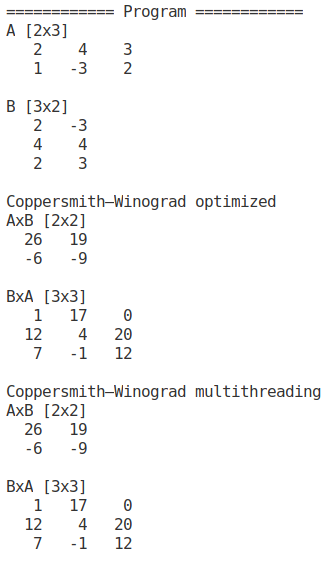
\includegraphics[width=0.4\textwidth]{4/inc/e1.png}
    \caption{Примеры работы программы}
    \label{fig:4.1}
\end{figure}


\begin{figure}[h]
    \centering
    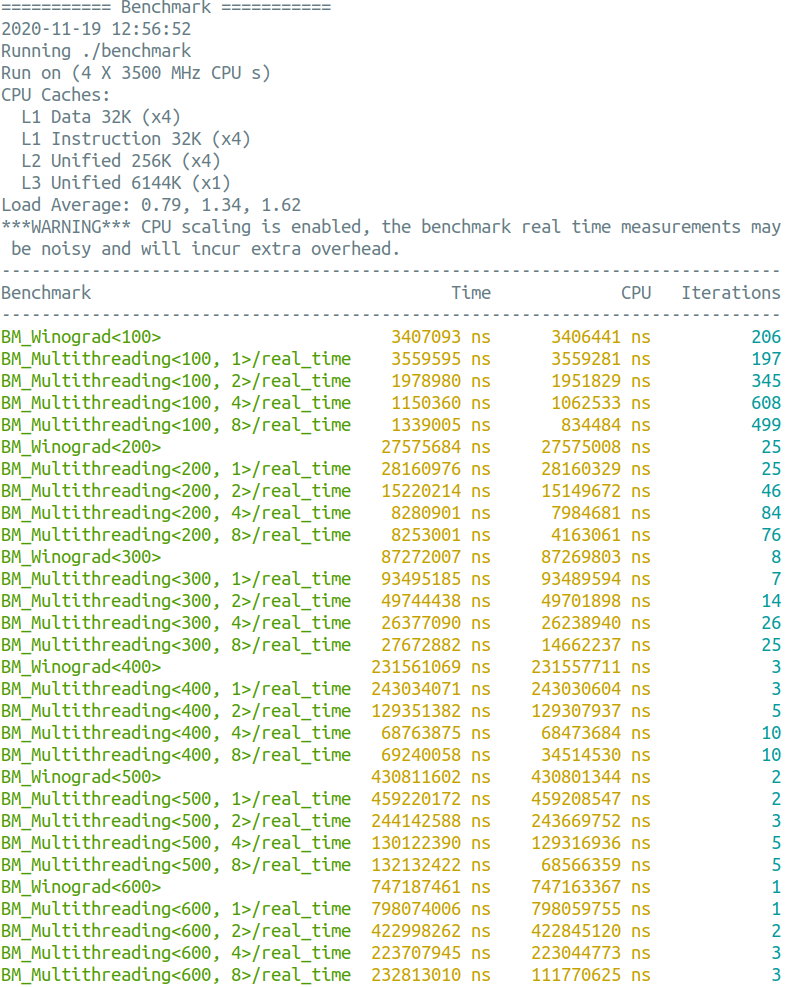
\includegraphics[width=0.8\textwidth]{4/inc/e2.png}
    \caption{Примеры работы программы}
    \label{fig:4.2}
\end{figure}

\pagebreak
\section{Результаты тестирования}

На рисунке \ref{fig:4.3} приведен результат теста с использованием фреймворка google test.

\begin{figure}[h]
    \centering
    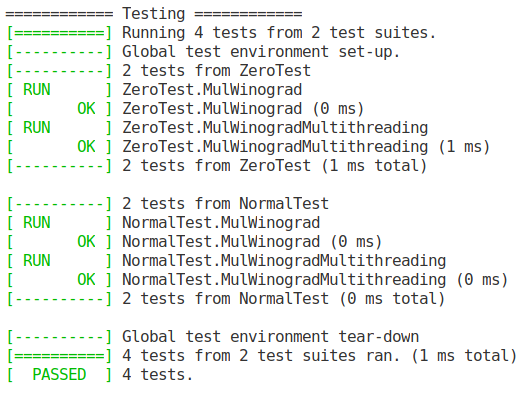
\includegraphics[width=0.6\textwidth]{4/inc/test.png}
    \caption{Результаты тестирования}
    \label{fig:4.3}
\end{figure}


% \section{Постановка эксперимента по замеру времени}
\pagebreak
\section{Сравнение времени работы}

В таблице \ref{tabular:benchmark} приведены замеры времени
работы алгоритмов умножения матриц на квадратных матрицах,
на основе них построены графики \ref{fig:4.3}.



% \def\arraystretch{1.2}
\setlength\tabcolsep{0.1cm}

\begin{table}[h]
    \centering
    \csvreader[tabular=|c|c|c|c|c|c|,
        table head=\hline
        \bfseries Размер
        & \bfseries Последо.
        & \bfseries 1 поток
        & \bfseries 2 поток
        & \bfseries 4 поток
        & \bfseries 8 поток
        \\\hline,
        late after line=\\\hline]
        {4/inc/benchmark.csv}{}
    { \csvcoli & \csvcolii & \csvcoliii & \csvcoliv & \csvcolv & \csvcolvi}
    % \csvautotabular{2/inc/benchmark2.csv}
    \caption{\label{tabular:benchmark} Времени работы (ns)}
\end{table}


\pagebreak
\begin{figure}[!h]
    \centering
    \begin{tikzpicture}
        \begin{axis}[
            scale=1.7,
            axis lines=left,
            xlabel=Размер матрицы,
            ylabel={Время, нс},
            legend pos=north west,
            xmajorgrids=true,
            ymajorgrids=true
        ]
            \addplot table[x=n,y=t0,col sep=comma] {4/inc/benchmark.csv};
            \addplot table[x=n,y=t1,col sep=comma] {4/inc/benchmark.csv};
            \addplot table[x=n,y=t2,col sep=comma] {4/inc/benchmark.csv};
            \addplot table[x=n,y=t4,col sep=comma] {4/inc/benchmark.csv};
            \addplot table[x=n,y=t8,col sep=comma] {4/inc/benchmark.csv};
            \legend{Последовательный, 1 поток, 2 поток, 4 поток, 8 поток}
        \end{axis}
    \end{tikzpicture}
    \caption{Зависимость времени работы алгоритмов умножения матриц от размеры матрицы и количество потоков}
    \label{fig:4.3}
\end{figure}


% \section{Сравнительный анализ на материале экспериментальных данных}
% эксперименты+выводы

\section{Вывод}

График показывает, что многопоточная версия более эффективна,
когда количество потоков увеличивается, производительность пропорциональна количеству потоков до тех пор,
пока она не станет равной количеству ядер процессора, и наиболее эффективна,
когда количество потоков равно количеству ядер процессора.
Затем, если количество потоков увеличивается, происходит небольшое уменьшение
из-за необходимости управлять большим количеством потоков.
